\clearpage{\pagestyle{empty}\cleardoublepage}

\chapter{Object reconstruction}\label{chap:objects}
%\section{Object reconstruction}\label{sec:objects}

After having described the ATLAS detector in Chapter~\ref{chap:atlas} 
and the procedure for Monte Carlo simulation of events in Chapter~\ref{chap:mc},
we understand that what we deal with when we talk about ``data'' 
is raw digital signals from the detector,
either the real one or the simulated one.

In the following Chapter we will explain how, starting from these outputs,
objects are reconstructed to be used in physics analyses~\cite{Aad:2009wy}. 
This process is what is called ``offline event reconstruction'' since
it is not done in real time, due to the time required by the algorithms
to perform their tasks.

In general we could describe the full procedure as subdivided into
three main steps: a pre-reconstruction stage where the electronic signals are
translated into measurements; a pattern-recognition step where the measurements
are assembled into the building blocks of particles, e.g. tracks and energy clusters;
a particle identification final leg where the full detector information elaborated 
is combined to match a candidate physics object 
(electrons, muons, jets and the missing transverse energy \met).

%In addition, some details from
%selections specific for the analyses presented in this dissertation will be given.

\section{Tracks}\label{sec:tracks}

Particle trajectories (``tracks'') are used both to reconstruct the particle itself, giving the 
momentum measurement, and to identify the interaction vertices.
The parameters describing a track are: $q/p$, the charge divided by the momentum; $\theta$, or more used $\eta$, the angle
with respect to the Z axis in the $R$Z plane measured from the 
perigee\footnote{The perigee is the point of the track closest to the origin.}; $\phi_0$, the angle 
with respect to the X axis in the XY plane measured from the perigee; $d_0$, the impact parameter, 
or perigee with respect to the Z axis in the XY plane; $z_0$, Z component of the perigee.
These parameters are shown in the double-view drawing of Figure~\ref{fig:trackpar}.

\begin{figure}[tb]\begin{center}
	\subfigure[]{
  	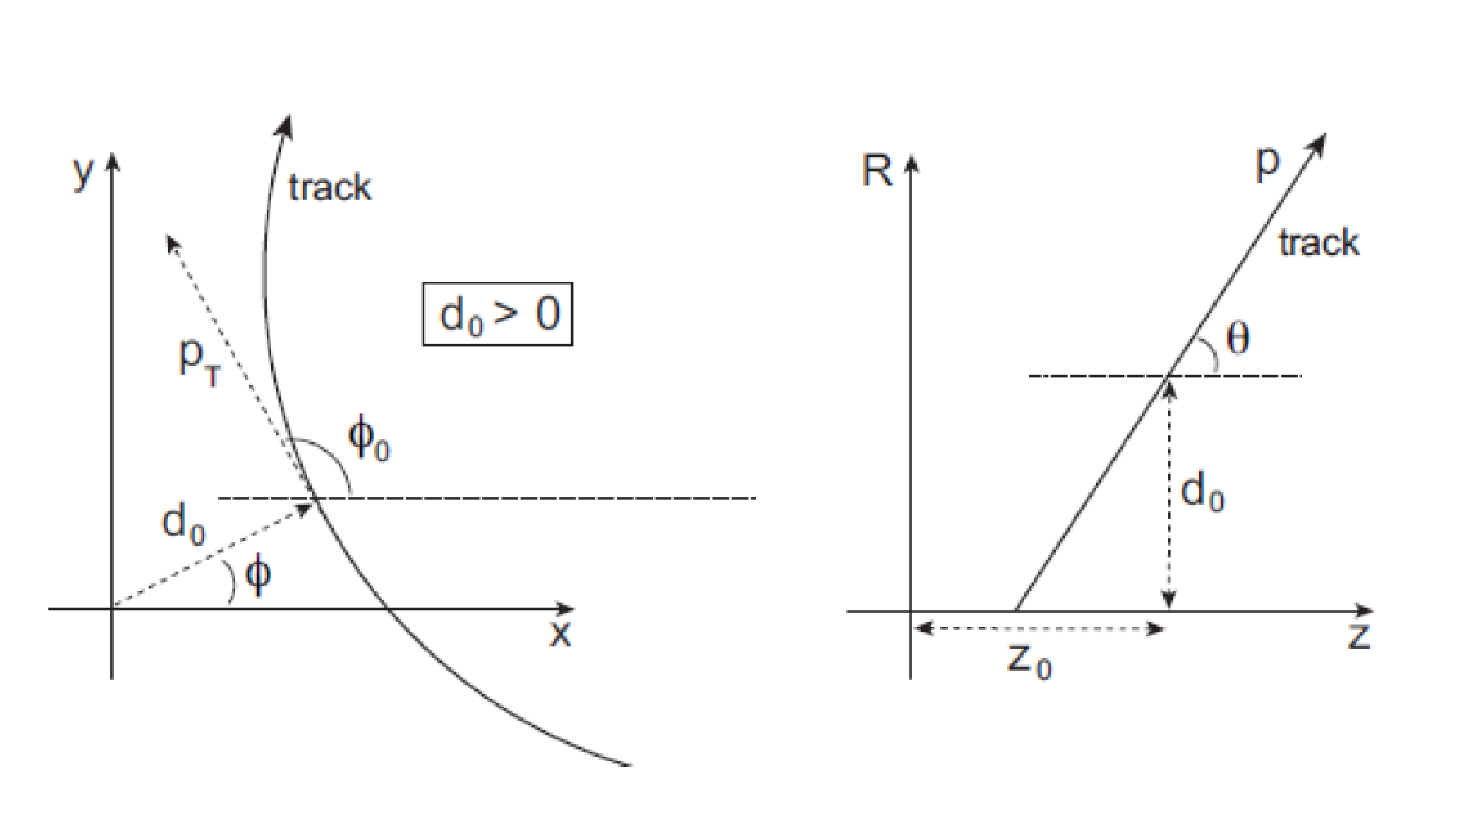
\includegraphics[width=0.7\textwidth]{objectsreconstruction/figures/tracks}}
	\caption[bla]{Schematic drawings of the parameters used for track reconstruction in the XY and $R$Z planes (left and right respectively)
          where the origin is the beam spot, i.e. where the protons collide and interact.
\label{fig:trackpar}}
\end{center}\end{figure}

In order to reconstruct the track, the first step is to retrieve the information from
the ID hits, which are converted into three-dimensional space points. Then, 
the {\it inside-out} algorithm~\cite{Cornelissen:1020106} is used, starting from a
seed of three aligned hits in the pixel detector or in the SCT.
From there, a path is formed along the seed directional information adding
space points one by one. This is done by using a Kalman filter algorithm~\cite{Frühwirth1987444}
which checks progressively the compatibility between the track (also progressively updated)
and the new point. The five track parameters described before are also computed at this step.

As basic requirements, the candidate track must be formed by at least seven points
measured in the silicon detectors, $d_0$ must be lower than 10~mm and the 
transverse momentum must be higher than 150~\mev.  A cleaning procedure then 
rejects incomplete tracks or tracks sharing hits with others, or composed by
false space points. The candidate tracks are extended
into the TRT and re-fitted taking into account the effects from the interaction
of the charged particle with the detector material. If at least ten TRT hits
within 10~mm from the extrapolated points the track is kept and re-fitted.

A second algorithm, called {\it outside-in}, is applied in order to better
reconstruct tracks from secondary charged particles. This algorithm does
the opposite of the inside-out one, taking as seeds hits in the TRT (the
ones not associated to any track candidate in by the inside-out reconstruction)
and extrapolating back to the SCT and pixel detector.


\section{Primary vertex}\label{sec:primaryvertex}

In general, a primary vertex (PV) is identified by the tracks associated to it.
The reconstruction is performed via an iterative procedure~\cite{ATLAS-CONF-2010-069}
starting from a seed defined as the maximum in the distribution of the $z_0$ parameter
of reconstructed tracks. After tracks are assigned to the PV with the aid of an
iterative $\chi^2$ fit, the ones that fall out of more than 7$\sigma$ from the PV
are used to seed another PV until no track is left without being assigned to a vertex
(one track can be associated to more than one vertex).

A PV must have at least two associated tracks and its position must be consistent with 
the beam collision region in the XY plane. The hard-scatter PV is chosen as the one
with the highest sum of squared transverse moments of the tracks. The other reconstructed PVs 
are identified with pile-up interactions. Another kind of vertices, not
compatible with the requirement of coming from close to the proton collision spot,
are the secondary vertices, originating from the decay of short-lived particles.
These vertices are useful to identify $B$-hadrons and will be described in Section~\ref{sec:btagging}.

As can be expected, high pile-up environments deteriorate the performance of vertex reconstruction,
as more fake tracks are introduced and nearby interaction might lead to the misreconstruction
of distinct vertices as a single one~\cite{ATLAS-CONF-2012-042}.

%\footnotetext{Of the reconstructed verteces consistently in the beam collision region in the XY plane with at least five associated tracks, the one with the highest number of tracks is taken as the primary one.}

\section{Electrons}\label{sec:electrons}
Electrons~\cite{eperf} are reconstructed for pseudorapidities up to $|\eta| = 2.5$, where
information from the ID is available, matching a track with an energy deposit
(cluster) in the electromagnetic calorimeter. 

Clusters~\cite{topocluster} are built starting from
$\Delta\eta\times\Delta\phi=0.025\times0.025$ single energy deposits summing
up into towers. Adjacent towers form clusters of $3\times7$ cells units in $\eta\times\phi$
in $|\eta|<1.4$ and $5\times5$ further. Of all the candidate reconstructed tracks,
those extrapolated to the calorimeter with the smallest $\dr$ with respect to the
energy cluster is chosen.

For our analyses, electrons in the transition region $1.37<|\eta_{\rm cluster}| <1.52$
with inactive material are excluded. Electrons are also required to have 
$\et = E_{\rm cluster}/\cosh\eta_{\rm track} > 25\gev$ and $z_0<2~$mm.
They have to be separated from any jet (Section~\ref{sec:jets}) selected by at least $\dr =0.4$.
90\% efficient isolation cuts to reduce the background from non-prompt electrons coming from
hadron decays are defined, one based on the energy from calorimeter cells surrounding the candidate in
a cone of radius $R=0.2$ and the other based on the track transverse momenta sum in a cone of radius $R=0.3$ around
the electron.

\section{Muons}\label{sec:muons}
%\subsection{Muons}\label{sec:muons}
Track segments reconstructed in the muon spectrometer are matched to tracks from the ID to build
muon candidates. The combined tracking information has to give $p_T>25\gev$ and $|\eta|<2.5$, and
$z_{0}$ has to be lower than 2~mm.
The muon radial distance from any selected jet is required to be $\Delta R > 0.4$.

A  $\pt$-dependent track-based isolation condition is defined as follows:
the scalar $\pt$ sum of all tracks (except for the muon track itself) 
in a cone of variable radius $R=10\gev/\pt^\mu$ around the lepton
must be less than 5\% of the muon $\pt$.
This isolation requirement works well also in high pile-up events
or in the case the muon is close to a jet.

\section{Jets}\label{sec:jets}
%\subsection{Jets}\label{sec:jets}

Jets from quark hadronization are reconstructed using the anti-$k_t$
algorithm~\cite{ref:Cacciari2008,ref:Cacciari2006,ref:fastjet} with a
radius parameter $R=0.4$ (from which the algorithm is often referred to as anti-$k_t$4) 
using calorimeter energy deposits\footnote{Topological clusters, abbreviated as ``topo-clusters'', are 
built from neighboring calorimeter cells starting from a seed deposit with a signal to noise ratio
higher than a certain threshold. Topo-clusters are treated as massless and their energy at the electromagnatic 
scale is the sum of the constituent cells.}
corrected for effects of non-compensation,
dead detector material and out-of-cluster leakage using local cluster calibrations~\cite{LCW1,LCW2}.

To subtract contributions from in-time and out-of-time pile-up interactions a correction is applied
parameterized according to the number of primary vertices in the event and the number of average interactions 
in the luminosity block ($<\mu>$) as a function of jet pseudorapidity.
Jets are finally calibrated to the hadronic scale using $\pt$- and $\eta$-dependent correction factors 
derived from Monte Carlo simulation~\cite{jes}.
For the analyses that we will present, only jets with $\pt > 25\gev$ and $|\eta| < 2.5$ are considered.

A variable called ``jet vertex fraction" (JVF) is defined as the fraction
of the sum of $\pt$ of tracks with $\pt>1\gev$
associated with the jet that comes from tracks originating from the primary vertex.
By requiring JVF$>0.5$ we avoid selecting jets from in-time pile-up events.

Since energy deposits from electrons can be reconstructed as jets, 
if jets are found within $\Delta R$ of 0.2 of a selected electron, the
jet closest to the lepton is discarded in order to avoid double-counting of electrons as jets.
After this one jet has been removed, electrons that lie within $\Delta R< 0.4$ of 
the jets remaining are removed.

\subsection{$b$-taggin}~\label{sec:btagging}

A technique to identify jets from the hadronisation of bottom quarks, 
called $b$-tagging~\cite{ref:ATLAS-CONF-2011-102}, is used. It
makes use of multivariate techniques combining the information
from secondary and tertiary decay vertices found within the jet
and from the impact parameters of displaced tracks to obtain a 
$b$-tagging weight that discriminates between $b$ and not-$b$
jets. A working point for this weight is chosen by finding
a compromize between a good efficiency (the ratio between tagged 
$b$-jets and true $b$-jets) and a high light-jet rejection
(the inverse of the number of light-jets misidentified as $b$-jets).
For our analyses, a working point corresponding to  70\% efficiency, 
$\sim$130 light-jet rejection and a charm-jet rejection of 5 is 
chosen\footnote{These values refer to jets with $\pt >20\gev$ and 
$|\eta|<2.5$ in simulated $t\bar{t}$ events.}


\section{Missing Transverse Energy}\label{sec:met}
%\subsection{Missing transverse energy}\label{sec:met}

To estimate the momentum of invisible particles in the event,
the missing transverse energy $\met$~\cite{met} is defined by first matching each calorimeter energy 
deposit with a high-$\pt$ lepton or jet. After the energies of these objects are
corrected accordingly to the respective calibration constants, the calorimeter clusters
that did not get associated with any  high-$\pt$ object are calibrated for energy losses in 
dead material regions and for the different response to the electromagnetic and hadronic
components of particle showers. Finally the \met\ is computed from the combinetion of the vector 
sum of the calibrated cluster momenta and a term associated with muon momenta.
